\documentclass[10pt]{article}
\usepackage{times}
\usepackage{fullpage}
\usepackage[left=0.8in,top=0.8in,right=0.8in,bottom=0.8in,nohead,foot=0.5in]{geometry}
\usepackage{listings}
\usepackage{balance}
\usepackage{graphicx} 
\usepackage{nameref}
\usepackage[margin=10pt,font=small,singlelinecheck=false,labelsep=period]{caption}
\usepackage{titlesec}
\titleformat{\section}{\large\bfseries}{\thesection}{1em}{}

\usepackage{color}

\lstdefinelanguage{chapel}
  {
    morekeywords={
      and, array, atomic,
      begin, bool, break,
      call, class, cobegin, complex, config, const, constructor, continue,
      def, distribute, do, domain,
      else, enum, except,
      for, forall,
      goto,
      if, imag, implements, in, int, inout, _invariant, iterator,
      let, like,
      module,
      nil, not,
      on, or, ordered, otherwise, out,
      param, _private, private, public,
      real, record, _release, repeat, return,
      select, serial, single, subtype, sync
      then, to, type, typeselect,
      uint, union, until, _unordered,
      var, _view,
      when, where, while, with,
      yield
    },
    sensitive=false,
    mathescape=false,
    morecomment=[l]{//},
    morecomment=[s]{/*}{*/},
    morestring=[b]",
}

\lstset{
    basicstyle=\footnotesize\tt,
    keywordstyle=\bf,
    commentstyle=\em,
    showstringspaces=false,
    flexiblecolumns=false,
    numbers=left,
    numbersep=5pt,
    numberstyle=\tiny,
    numberblanklines=false,
    stepnumber=0
  }

\newcommand{\chpl}[1]{\lstinline[language=chapel,basicstyle=\normalsize\tt,keywordstyle=]!#1!}

\lstnewenvironment{chapel}{\lstset{language=chapel,xleftmargin=2pc}}{}


\newcommand{\ie}{\emph{i.e.}}
\newcommand{\eg}{\emph{e.g.}}

\newfont{\affaddr}{phvr at 10pt}
\newfont{\affaddrit}{phvro at 10pt}

\setlength{\parskip}{5pt}
\setlength{\parindent}{0pt}

\title{Chapel Compiler Overview}

\author{Steve Deitz}

\date{June, 2010}

\begin{document}

\maketitle

\begin{quote}
\footnotesize
{\bf An important caveat.}  This document attempts to explain how the
Chapel compiler works.  It is most certainly incomplete and wrong.
\end{quote}

\section{Introduction}

This document contains rough notes about the state of the compiler in
June of 2010.  It is subdivided into three sections.
Section~\ref{sec:ast} describes the intermediate representation,
sometimes referred to as the AST.  Section~\ref{sec:passes} describes
the passes and assumptions that may be made about the AST before and
after the various passes.  Section~\ref{sec:misc} covers miscellaneous
topics.

This document assumes the reader has excellent familiarity with the
Chapel language.

\section{Intermediate Representation}
\label{sec:ast}

The intermediate representation (IR), alternatively called the AST, is
a graph-like structure defined by instances of subclasses of the
Symbol, Type, and Expr classes (which are themselves subclasses of the
BaseAST class).  This representation is used throughout the entire
compilation process, though assumptions on its structure change.  (For
example, after normalization, CallExprs will not be nested with the
exception of a CallExpr that represents the MOVE primitive (C
assignment).)  The BaseAST, Symbol, Type, and Expr classes are never
instantiated.

This graph is rooted at the module rootModule which contains DefExprs
of all the modules in the program, as well as literals and other
global entities.

Nodes in the representation can also be accessed via global vectors of
each node type.  These vectors are named as \cc{gASTs} where \cc{AST}
is a particular AST node type.  For example, \cc{gFnSymbols} is a
vector of all of the functions in a program, nested or not.  Newly
constructed nodes are automatically added to these vectors by their
constructors.  Between passes, these vectors are pruned of all AST
nodes that are not part of the IR (part of the graph).

Three vectors of modules also capture the modules that make up the
AST.  The vector \cc{allModules} is a vector of all the modules, and
is probably identical to \cc{gModuleSymbols}.  The vector
\cc{userModules} contains all of the user modules.  For debug
purposes, this is useful for looking at the test code in question.
The vector \cc{mainModules} contains all of the main modules.  See
Section~\ref{sec:modulesymbol} for more information on modules.

\subsection{BaseAST}

Every node in the AST is a subclass of BaseAST.  The BaseAST class
contains three fields:
\begin{itemize}
\item \cc{AstTag astTag} is an enumeration value used to identify a
  node's dynamic type.  It is accessed via macros \cc{isAST} and
  \cc{toAST}, where \cc{AST} is replaced by a node type, to check if a
  node is a particular type or to safely cast it to such a type (NULL
  if it is not such a type).  This cast mechanism is used instead of
  C++'s \cc{dynamic_cast} mechanism.

\item \cc{int id} is a unique integer assigned during construction.
  This is useful for debugging as each AST node will be numbered based
  on the order of construction.  These numbers start at 1.  During
  debugging with gdb via the --gdb flag, you can use the call aid(id)
  to get a pointer to an AST node based on this number.

\item \cc{int lineno} stores the line number of the Chapel code that
  this AST node originated from.  During parsing, this field is set
  based on YACC state.  Afterwards, these numbers are set based on the
  global variable \cc{currentLineno}.  This line number can be changed
  using the macro \cc{SET_LINENO(ast)} which will set the global line
  number to the line number associated with a given AST node.  Thus,
  for example, if you are adding a compiler-inserted CallExpr before
  an existing CallExpr in the AST, you can set the global line number
  to that of the existing CallExpr, and the new compiler-inserted AST
  nodes will use the same line number.
\end{itemize}

As a note for improvement, our line numbers are often incorrectly
reported.  If \cc{SET_LINENO} were used more consistently, this would
not be the case.  One way to improve things would be to generate an
internal error if \cc{SET_LINENO} were not used correctly.  To do
this, we would want to unset the line number somehow.  We could do
this with an \cc{UNSET_LINENO} macro or we could make the
\cc{SET_LINENO} macro require us to open a scope.  Then when we leave
this scope, we could set the current line number back to what it was
before we opened this scope (and unset at the outermost level).

\subsection{Symbol}

The Symbol group of AST nodes derive from the class Symbol.
Variables, constants, parameters, literals, arguments, fields, types,
enumeration symbols, modules, and labels are all represented by
symbols in the AST.

The fields in Symbol are:
\begin{itemize}
\item \cc{const char* name} stores the Chapel name of the symbol.
  This is used during scope resolution and function resolution to
  resolve unresolved symbol uses (UnresolvedSymExprs).  Comparing this
  field does not require a string comparison as it is canonicalized
  (see note on strings in Section~\ref{sec:strings}).
\item \cc{const char* cname} stores the name that we will generate in
  C.  This name is sometimes set during compilation to improve the
  readability of the generated code.  During the codegen pass, we
  legalize these names and mangle them as necessary.  Comparing this
  field does not require a string comparison as it is canonicalized
  (see note on strings in Section~\ref{sec:strings}).
\item \cc{Type* type} stores the resolved type of variables,
  arguments, and fields.  This is generally set during function
  resolution when types are resolved.  Before such resolution, the
  type \cc{dtUnknown} is used.
\item \cc{DefExpr* defPoint} points to a \cc{DefExpr}, the expression
  hook in the AST.  Every symbol has a DefExpr that connects the
  symbol to the AST.  The symbol can also show up in the AST via the
  expression \cc{SymExpr}.  These account for both defs (writes to the
  symbols) and uses (reads of the symbols).
\item \cc{std::bitset<NUM_FLAGS> flags} is a bit vector of flags
  (referred to as pragmas when they appear in Chapel code).  Flags are
  associated only with symbols.  See Section~\ref{sec:flags} for more
  information about flags.
\end{itemize}

The subclasses of Symbol include the following:
\begin{itemize}
\item VarSymbol (Section~\ref{sec:varsymbol})
\item ArgSymbol (Section~\ref{sec:argsymbol})
\item TypeSymbol (Section~\ref{sec:typesymbol})
\item FnSymbol (Section~\ref{sec:fnsymbol})
\item EnumSymbol (Section~\ref{sec:enumsymbol})
\item LabelSymbol (Section~\ref{sec:labelsymbol})
\item ModuleSymbol (Section~\ref{sec:modulesymbol})
\end{itemize}

\subsubsection{VarSymbol}
\label{sec:varsymbol}

The VarSymbol class represents variables, including both global
variables (in a module) and local variables (in a function).  The
VarSymbol is used for fields (in a type).

The constness of a variable is handled via a flag, so constants and
parameters (compile-time constants) are represented by VarSymbol
objects as well.

The fields of VarSymbol include the following:
\begin{itemize}
\item \cc{Immediate* immediate} stores a representation of a literal
  symbol.  For example, 1 is an integer literal.  The representation
  of immediates is code that from IF1, an iterative flow analysis
  engine.
\end{itemize}

\subsubsection{ArgSymbol}
\label{sec:argsymbol}

The ArgSymbol class is used to represent the formal arguments of
functions.  The fields of the ArgSymbol include the following:
\begin{itemize}
\item \cc{IntentTag intent} stores the specified intent of the
  argument.  This can be blank, in, inout, out, or const.  Note that
  \cc{INTENT_REF} does not appear to be used and probably predates the
  introduction of reference types.  The intent field also marks
  generics via parameter and type intent arguments.  The intent field
  is largely ignored after function resolution, which is to say that
  the functionality of the intent has been folded into the
  representation without it.  Thus if the intent were inout, then a
  copy in and a copy out (via assignment and/or a move primitive)
  would have been added to the AST.
\item \cc{BlockStmt* typeExpr} stores the type of the argument as it
  is parsed in.  This specified type is resolved during function
  resolution when the \cc{type} field is set.  After the \cc{type}
  field is set, this field is ignored.
\item \cc{BlockStmt* defaultExpr} stores the expression specified as a
  default for the argument (what is used if no actual is specified).
  The default expression is folded into the AST during function
  resolution by creating a default wrapper function.
\item \cc{BlockStmt* variableExpr} stores the expression specified
  after an ellipsis specifying a variadic argument.  This must resolve
  during function resolution to a parameter expression (it can also be
  omitted for variadic arguments or a query identifier).  After
  function resolution, this field is ignored.
\item \cc{Type* instantiatedFrom} stores the argument from which this
  argument has been instantiated.  That is, it points to the original
  argument in a generic function.  It is only used during the function
  resolution pass.
\item \cc{bool instantiatedParam} marks an argument as a parameter
  that has been instantiated.  This is only used during function
  resolution, and should most likely be a flag, or a hash table.
\item \cc{bool markedGeneric} marks an argument as generic
  (presumably).  It is used to mark a type as generic if the Chapel
  programmer inserts a ? next to a generic type that has default
  values for all of its generic fields.  This is also used to mark
  arguments when building default functions, but I'm not sure why.
  This should probably be a flag.  It does span multiple passes (being
  set in normalize and used in resolution).
\end{itemize}

\subsubsection{TypeSymbol}
\label{sec:typesymbol}

The TypeSymbol class is used for types.  The subclasses of Type can be
thought of as storing auxillary information about types.  There is a
one-to-one mapping between TypeSymbols and Types.  So the \cc{type}
field of TypeSymbol points to a subclass of Type, and the \cc{symbol}
field of this type class will point back at the TypeSymbol.

A good refactoring would probably be to use TypeSymbol everywhere that
Type is used.  Then a field in TypeSymbol could point to its auxillary
information, but we would never have to point back.  This refactoring
would require changing, for example, the \cc{type} field of Symbol
from Type to TypeSymbol.

The TypeSymbol class has no fields, inheriting all of the information
it needs from the Symbol class, and putting all of the extra
information in the Type class.

\subsubsection{FnSymbol}
\label{sec:fnsymbol}

The FnSymbol class is used to represent all methods and functions in a
program.  Top-level code in ModuleSymbols is moved into FnSymbols
(their initialize functions pointed to by initFn in ModuleSymbol)
during parsing.

The fields of FnSymbol include the following:
\begin{itemize}
\item \cc{AList formals} is an alist (linked list of Expr subclasses)
  of DefExprs that define ArgSymbols.  These are the formal arguments
  stored in a specified order.
\item \cc{DefExpr* setter} is non-null for var functions, and
  represents the setter argument.  This argument is of bool type and
  is set to true only when the function is used in an lvalue setting.
  The implementation of var functions involves cloning the function so
  that there are two versions, one for lvalues and one for
  non-lvalues.  However, it is important to note that at function
  resolution time, we don't determine which is called.  That is, we
  always resolve both versions.  So this argument can not be used as a
  parameter.
\item \cc{Type* retType} stores the resolved return type of a
  function.  This field is set during function resolution because only
  at that point can we determine the type.
\item \cc{BlockStmt* where} stores the expression that is the where
  clause for a function.  It is evaluated to true or false during
  function resolution when choosing a candidate.  This has language
  ramifications to our in-order function resolution since we could end
  up in an infinite recursion if we have to evaluate a where clause by
  evaluating a function that we have not yet finished evaluating.
  This results in an error rather than an infinite recursion.
\item \cc{BlockStmt* retExprType} stores the specified return type as
  an expression.  The type cannot be resolved from this expression
  until function resolution time, except for simple cases.  This
  expression is looked at during normalization when normalizing
  returns (making each function have a single return statement that is
  the last statement in that function).
\item \cc{BlockStmt* body} stores the BlockStmt that is the body of
  the function.  This is where the code is!
\item \cc{IntentTag thisTag} stores an intent on the implicit this
  argument.  It is set during parsing before the implicit this
  argument has been created.  Perhaps we could also create the
  implicit this argument earlier...
\item \cc{RetTag retTag} stores the return tag, whether this function
  is a var function, a param function, a type function, or a regular
  ``value'' function.
\item \cc{IteratorInfo* iteratorInfo} stores information about the
  iterator record and class that are created when an iterator function
  is lowered into a record and a class with methods during the
  lowerIterators pass.  The prototypes are set up during function
  resolution, and then filled in when iterators are lowered.
\item \cc{Symbol* _this} stores a pointer to the implicit this
  argument for methods.  For constructors, \cc{_this} is a VarSymbol
    that is declared in the body of the constructor.
\item \cc{Symbol* _outer} pertains to outer classes.  It is set for
  nested class constructors and replaces \cc{_this}.
\item \cc{FnSymbol *instantiatedFrom} is set for functions that have
  been instantiated from generic functions.  This points to the
  generic function, is only used during function resolution, and can
  probably be stored in a hash table.
\item \cc{SymbolMap substitutions} is a hash table of the
  substitutions that were made to instantiated this generic function.
  The keys are arguments in the generic function (original function)
  and the values are the types or parameters over which these
  arguments have been instantiated.
\item \cc{BlockStmt* instantiationPoint} points to a point in the code
  that we are using as the instantiation point for function resolution
  (just like the instantiation point in C++).  Constrained generics
  will not need an instantiation point!
\item \cc{Vec<BasicBlock*>* basicBlocks} is built when calling
  buildBasicBlocks on a function.  The basic block is stored as a
  vector of Exprs where these are pointing at the expressions in the
  function.  Basic blocks are used by the dataflow analyses and
  optimizations.  They are not maintained.  This probably just does
  not need to be a field, as it is not updated and is recomputed for
  each analysis.
\item \cc{Vec<CallExpr*>* calledBy} points to all of the CallExprs
  that call this function.  These vectors are computed by
  \chpl{compute_call_sites}, but are not mainted when CallExprs are
  changed.  This field could be removed if this function were to build
  a Map from FnSymbols to a vector of CallExprs.
\item \cc{const char* userString} is set during parsing so that we can
  store the prototype of the function and issue error messages to the
  user that display function candidates just as they are written in
  the Chapel code.
\item \cc{FnSymbol* valueFunction} points to a value version of a var
  function.  This is only referenced in function resolution and the
  pass that culls references.  It may be better to use a hash table
  defined and used by the resolution passes.
\end{itemize}

\subsubsection{EnumSymbol}
\label{sec:enumsymbol}

The EnumSymbol class defines an enumeration constant (not an
enumeration type).  This class has no fields, inheriting all of the
information it needs from the Symbol class.

\subsubsection{LabelSymbol}
\label{sec:labelsymbol}

The LabelSymbol class defines a label that can be the target of a
break or continue statement, or a goto statement.  There are no goto
statements in Chapel, but there are goto statements in our
intermediate representation, and they are introduced especially
(perhaps only) when iterators are lowered into classes and methods
(including an advance method).  In subsequent calls to the advance
method, a jump table is implemented with goto statements.

The DefExpr of the LabelSymbol must be declared in a function and is
eventually the target of a goto.  During scope resolution, all break
and continue statements are lowered to normal goto statements.  The
SymExpr of a LabelSymbol becomes a use of the label.  Such uses only
occur in GotoStmts.

This class has no fields, inheriting all of the information it needs
from the Symbol class.

\subsubsection{ModuleSymbol}
\label{sec:modulesymbol}

Chapel programs are composed of modules and these modules are stored
in the ModuleSymbol.  The fields of ModuleSymbol include the
following:
\begin{itemize}
\item \cc{ModTag modTag} categorizes the type of module as a user
  module, an internal module, a main module (passed to the compiler
  explicitly, and thus a candidate for main, I think), or a standard
  module.
\item \cc{BlockStmt* block} contains the code defined in a module
  symbol.  This is mostly a list of DefExprs of functions, types, and
  global variables.
\item \cc{FnSymbol* initFn} contains a pointer to the initialize
  function for a module.  This function is called when a module is
  used at program startup.  During the parse pass, it is built and the
  executable code at module level is moved into this function.
\item \cc{const char* filename} stores the filename that this module
  was declared in.  Historically, we used to store filename alongside
  lineno, but this seemed like overkill given that all of the AST in a
  module has the same filename.  After inlining, this may not be the
  case, but the current way may be sufficient.
\item \cc{Vec<ModuleSymbol*> modUseList} is a vector of modules used
  to determine the order of module initialization. (bradcray r15954)
\item \cc{Vec<ModuleSymbol*> modUseSet} is a vector of modules used to
  determine the order of module initialization.  Presumably, this
  field is a set and the previous one is a vector.  It is unclear
  whether these have to be fields. (bradcray r15954)
\end{itemize}

\subsection{Type}

Type is basically a class that is associated with TypeSymbols in a
one-to-one mapping and stores auxillary information relevant to the
particular kind of type.

The fields in Type are:
\begin{itemize}
\item \cc{Vec<Type*> dispatchParents} stores the vector of types that
  are parents, \eg, a class's superclasses.
\item \cc{Vec<Type*> dispatchChildren} stores the vector of types that
  are children, \eg, a class's subclasses.  The inheritance
  relationship is set up before resolving symbols via scope resolution
  since we need to know this relationship within methods.  Note that
  the compiler, to date, only supports a single parent though we use a
  vector here for future support of multiple inheritance.
\item \cc{Type* scalarPromotionType} marks the element type for which
  this type would scalar promote a function.
\item \cc{TypeSymbol* symbol} points to the TypeSymbol that represents
  this type and points to this class via the \cc{type} field.
\item \cc{Symbol* defaultValue} points to a symbol that can be used to
  initialize a variable of this type.  If \cc{defaultValue} is
  \cc{NULL} (as in the case of a record), then the default constructor
  is invoked to initialize a variable of this type.
\item \cc{FnSymbol* defaultConstructor} points to the default
  constructor for this type.  The default constructor is fairly
  elaborate in Chapel, having an argument for every field.  Even if a
  type is defined with user-defined constructors, we still create and
  call the default constructor when resolving the type.  However, the
  default constructor is deprioritized.
\item \cc{FnSymbol* defaultTypeConstructor} points to the default type
  constructor.  This name is less than ideal since there are never any
  type constructors other than the default type constructor.  The type
  constructor is resolved to when specifying a type rather than
  instantiating an instance of the type.  For classes that have fields
  where the type of the field is omitted, the type constructor will
  expect a type for this field whereas the default constructor will
  expect a value.  This implements the semantics which allow for a
  class like \chpl{class C \{ var x; \}} to be constructed with a call
  to the type constructor as \chpl{C(int)}.
\item \cc{FnSymbol* destructor} points to a destructor.  This field is
  not set until during function resolution and is then used during the
  pass that inserts calls to the destructors.
\item \cc{Vec<FnSymbol*> methods} is a vector of the methods on a
  type (including primitive types).
\item \cc{bool hasGenericDefaults} marks a type if all of the generic
  fields on the type have default values, since such a type has to be
  handled with care if the generic version is sought (via a ?).
\item \cc{Type *instantiatedFrom} points to the generic type from
  which this type was instantiated.
\item \cc{SymbolMap substitutions} is a hash table of the
  substitutions that were made to instantiate this generic type.  It
  is similar to the field on the function symbol.
\item \cc{ClassType* refType} points to the reference type if this
  type is a value type.  Reference types are introduced during
  function resolution because there are no reference types in Chapel,
  just in the intermediate representation.
\end{itemize}

The subclasses of Type include the following:
\begin{itemize}
\item PrimitiveType (Section~\ref{sec:primitivetype})
\item EnumType (Section~\ref{sec:enumtype})
\item ClassType (Section~\ref{sec:classtype})
\end{itemize}

\subsubsection{PrimitiveType}
\label{sec:primitivetype}

The PrimitiveType class is used to represent nodes that are primitive
types such as integers, reals, strings, C files, a timer type, some
auxillary types for sync and single variables, etc.

This class has no fields, inheriting all of the information it needs
from the Type class.

\subsubsection{EnumType}
\label{sec:enumtype}

The EnumeratedType class contains auxillary information for enumerated
types, basically a list of EnumSymbol constants.  The fields in
EnumType are:
\begin{itemize}
\item \cc{AList constants} is a list of DefExprs that define the
  EnumSymbols for this enumerated type.
\end{itemize}

\subsubsection{ClassType}
\label{sec:classtype}

The ClassType class contains auxillary information for classes,
records, and unions.  The fields of ClassType are:
\begin{itemize}
\item \cc{ClassTag classTag} is an enumeration to identify whether
  this ClassType is a class, record, or union.  The creative constant
  name \cc{CLASS_CLASS} suggests this class could have a better name.
\item \cc{AList fields} is a list of DefExprs that define the fields
  in this class, represented as VarSymbols.
\item \cc{AList inherits} is a list of Exprs that represent the types
  from which this type inherits.  In the current implementation this
  is limited to a SymExpr.  Inheriting from generics is complicated
  because we do not instantiate generic types until function
  resolution, but we need to build up the inheritance hierarchy in
  time for scope resolution.  This poses a challenge, but we should be
  able to handle it by computing a generic inheritance graph.
\item \cc{Symbol* outer} points to the outer class if this is an inner
  class.
\end{itemize}

\subsection{Expr}

The Expr subclasses represents the structure of the program in the
AST.  There may be multiple pointers to the same instances of Symbol
or Type subclasses, but there is only a single instance of a pointer
to any Expr subclass, with the notable exception of back pointers such
as \cc{parentExpr} and \cc{defPoint}.  The back pointer
\cc{parentSymbol} is to a symbol and so is not quite as exceptional.

To elaborate, all occurrences of symbols are wrapped by a unique
SymExpr instance.  So given a program that contains the calls
\begin{chapel}
f1(a, b);
f2(b, c);
\end{chapel}
the AST for this portion of the program will be represented
(throughout the entire compilation) by two different instances of
CallExpr.  Each instance will have the \cc{baseExpr} field point to a
distinct instance of the SymExpr class.  The \cc{var} fields will
point to the FnSymbol instances that represent \chpl{f1} and
\chpl{f2}.  Each instance of CallExpr will have the \cc{argList} field
point to a list of expressions.  Each list will contain two distinct
SymExpr instances, for a total of four distinct SymExpr instances.
The second SymExpr instance in the first CallExpr will set \cc{var} to
point to the Symbol that represents \chpl{b}, as will the first
SymExpr instance in the second CallExpr.  Thus the symbol pointer
appears more than once via ``forward'' pointers, but pointers to Expr
subclasses can appear only once via ``forward'' pointers.

The fields in Expr are:
\begin{itemize}
\item \cc{Expr* prev} is a back pointer to the previous expression in
  a list, if this expression is in a list.
\item \cc{Expr* next} is a pointer to the next expression in a list,
  if this expression is in a list.  It may be useful to think of next
  as a back pointer if we think of the ``forward'' pointer to the
  AList as pointing to all of the expressions in the list.
\item \cc{AList* list} is a back pointer to the list of expressions to
  which this expression is a part.
\item \cc{Expr* parentExpr} is a back pointer to the parent
  expression.  This is set any time an Expr is pointed to by another
  Expr.  For example, a parent CallExpr node points to its children
  via \cc{baseExpr} and \cc{argList}.  The Expr nodes pointed to via
  these pointers will set \cc{parentExpr} to point to this parent
  CallExpr node.  The \cc{parentExpr} node can be \cc{NULL} even if
  this node is part of the AST.  This happens if this Expr node is
  pointed at directly from a Symbol or Type node.  For example, via
  the \cc{body} field of a FnSymbol node.
\item \cc{Symbol* parentSymbol} is a back pointer to the parent
  symbol.  If this is not set, the node is not considered part of the
  AST.  When using \cc{remove} to remove an expression from the AST,
  all the Expr nodes that make up that expression are traversed and
  their \cc{parentSymbol} back pointers are set to NULL.  Testing for
  the existence of \cc{parentSymbol} is sufficient to tell if an Expr
  node is part of the AST.  Between passes, nodes that are not part of
  the AST are garbage collected.
\end{itemize}

Note that by and large, \cc{prev}, \cc{next}, \cc{list} do not have to
be manipulated because inserting and removing Expr nodes from the AST
should be done via the functions \cc{insertAtHead}, \cc{insertAtTail},
\cc{insertBefore}, \cc{insertAfter}, \cc{replace}, and \cc{remove}.
These functions will also update the back pointers \cc{parentExpr} and
\cc{parentSymbol}, which should never be set elsewhere.

The subclasses of Expr include the following:
\begin{itemize}
\item DefExpr (Section~\ref{sec:defexpr})
\item SymExpr (Section~\ref{sec:symexpr})
\item UnresolvedSymExpr (Section~\ref{sec:unresolvedsymexpr})
\item CallExpr (Section~\ref{sec:callexpr})
\item NamedExpr (Section~\ref{sec:namedexpr})
\item BlockStmt (Section~\ref{sec:blockstmt})
\item CondStmt (Section~\ref{sec:condstmt})
\item GotoStmt (Section~\ref{sec:gotostmt})
\end{itemize}

Note that some of these end with ``Stmt'' while others end with
``Expr.''  This distinction is important as, at least after
normalization, we will never get to a BlockStmt when traversing the
AST from SymExpr, UnresolvedSymExpr, CallExpr, or NamedExpr if we do
not traverse into Symbol nodes unless we are coming from a DefExpr
node and we do not traverse into Type nodes unless we are coming from
a TypeSymbol node.  This is indeed how AST traversal works.  See
Section~\ref{sec:traverse}.

\subsubsection{DefExpr}
\label{sec:defexpr}

Every symbol, with the exception of \cc{rootModule}, is pointed to by
a distinct instance of the DefExpr class.  The forward pointer to this
DefExpr locates the declaration of this symbol in the AST.

The fields in DefExpr are:
\begin{itemize}
\item \cc{Symbol* sym} is a pointer to the symbol that this DefExpr
  declares.  Note that using the typical terminology of compilers,
  this is not a def for a VarSymbol after normalization.  A def would
  be marked by a SymExpr (an occurrence of the symbol) that is on the
  left-hand side of an assignment or primitive move, for example.
\item \cc{Expr* init} is used to capture an expression that is used to
  initialize this symbol.  For variables and fields, this is the
  initialization expression in the Chapel code.  This is not used for
  ArgSymbols (where the corresponding expression is pointed to
  directly by the ArgSymbol field \cc{defaultExpr}).  After
  normalization, this field should be \cc{NULL} and the AST should be
  modified so that the functionality is elsewhere.  For variables,
  this means that there will be expressions inserted after this
  DefExpr to do the initialization.  For fields, this means that there
  will be expressions added to a default constructor to do the
  initialization.  The code to complete this transformation is in the
  normalize pass.
\item \cc{Expr* exprType} is used to capture an expression that is
  used to specify the type.  Before function resolution, the type is
  stored as an expression.  It could be a simple SymExpr if the type
  is a simple record \chpl{R} or a primitive type like \chpl{int}, but
  this need not be the case if the type is specified as a call to a
  type function or an instantiated type such as \chpl{C(int)}.  The
  \cc{exprType} field undergoes similar transformations to the
  \cc{init} field at the same time (normalization).
\end{itemize}

\subsubsection{SymExpr}
\label{sec:symexpr}

Whenever a symbol is used or defined (not declared) in the AST, it is
wrapped by an instance of the SymExpr class.  This makes for a bulky
intermediate representation.  An optimized intermediate representation
might replace the list of expressions in a normalized CallExpr by a
vector of Symbols.

The fields in SymExpr are:
\begin{itemize}
\item \cc{Symbol* var} is a pointer to the occurrence of the symbol
  that this SymExpr wraps.  Later in compilation, it is often useful
  to categorize these SymExprs as either uses or defs.  I think there
  is a slight problem with respect to this categorization as currently
  involves references.
\end{itemize}

\subsubsection{UnresolvedSymExpr}
\label{sec:unresolvedsymexpr}

The UnresolvedSymExpr nodes represent names of symbols that have not
yet been resolved by either scope resolution (variables, fields,
arguments, etc.) or function resolution (functions).  This is one of
the most recently introduced nodes as it replaces UnresolvedSymbol, a
subclass of Symbol.

The fields in UnresolvedSymExpr are:
\begin{itemize}
\item \cc{const char* unresolved} is the name of a symbol for which
  the symbol has not been resolved.  Nodes of this type should not
  exist after function resolution.  They are eliminated during scope
  resolution and function resolution.  Comparing this field does not
  require a string comparison as it is canonicalized (see note on
  strings in Section~\ref{sec:strings}).
\end{itemize}

\subsubsection{CallExpr}
\label{sec:callexpr}

The CallExpr node represents function calls as well as primitive
calls.  Primitives are further explained in
Section~\ref{sec:primitives}.

The fields in CallExpr are:
\begin{itemize}
\item \cc{Expr* baseExpr} is a pointer to the base expression (the
  expression that evaluates eventually to a FnSymbol).  After function
  resolution, this field, if set, will always point to a SymExpr that
  points to a FnSymbol.  Before function resolution, there are
  additional possibilities.  For example, given the Chapel code
  \chpl{f()()}, where the call \chpl{f()} returns an instance of a
  class with a \chpl{this} metho, then the CallExpr of \chpl{f()} will
  be pointed to by the \cc{baseExpr} field.
\item \cc{AList argList} is a pointer to the expression list that
  makes up the actual arguments to this CallExpr.
\item \cc{PrimitiveOp* primitive} is a pointer to the primitive.  If
  this field is set, then \cc{baseExpr} will be \cc{NULL}.  It's a
  one-or-the-other situation.
\item \cc{bool partialTag} handles the case involved with resolving
  the Chapel code given by \chpl{x.y()} by marking this case.  We have
  to deal with two situations.  The first is where we are invoking a
  method \chpl{y}.  The second is where we are invoking a
  parenthesesless method (possibly a getter for a field) that returns
  a class instance with a \chpl{this} method, and then we are invoking
  the \chpl{this} method.  So in the latter case, we invoke two
  functions, while in the former case, we invoke just one.  This code
  is represented as a nested CallExpr, and the inner CallExpr is
  marked with this tag after normalization.
\item \cc{bool methodTag} marks basic method invocations, even if they
  are parenthesesless.  For example, with \chpl{x.y}, the method call
  of \chpl{y} after normalization will be mark this flag true, but
  \cc{partialTag} will not be marked true.  There are no nested call
  expressions.  It seems that if \cc{partialTag} is set, then
  \cc{methodTag} is set.
\item \cc{bool square} marks function calls that are invoked using
  square brackets.  This is the only distinguishing mark for this
  case.
\end{itemize}

\subsubsection{NamedExpr}
\label{sec:namedexpr}

The NamedExpr class is used to represent passing an actual to a
function via a named argument.

The fields in NamedExpr are:
\begin{itemize}
\item \cc{const char* name} is the name of the formal argument.
  Comparing this field does not require a string comparison as it is
  canonicalized (see note on strings in Section~\ref{sec:strings}).
\item \cc{Expr* actual} is the actual expression passed to the call.
\end{itemize}

\subsubsection{BlockStmt}
\label{sec:blockstmt}

The BlockStmt class represents a block of code in Chapel, including
all loops.

The fields in BlockStmt are:
\begin{itemize}
\item \cc{BlockTag blockTag} marks the BlockStmt with a tag.  This
  field used to be used to distinguish the different types of
  BlockStmts more than it is used now.  Most of this functionality has
  been moved into the blockInfo field via a CallExpr with a primitive.
  The remaining tags can be moved there as well, eliminating this
  field.  These tags mark this block in two ways.  First, scopeless
  blocks are marked to indicate that this block should not be
  considered relevant when completing scope resolution.  Second, type
  blocks are marked to indicate that the code in this block statement
  should only be used to determine the types of variables (during
  function resolution).  Such blocks are removed after function
  resolution and the code represented by this block is not executed.
\item \cc{AList body} is a list of expressions that form the body of
  this block, the statements within it.
\item \cc{CallExpr* blockInfo} is a call to a primitive that marks
  this block as special in some way, \eg, a while loop.
\item \cc{CallExpr* modUses} is a call of ModuleSymbols where each of
  these ModuleSymbols represents a use of a particular module.  This
  list is largely constructed during scope resolution.
\item \cc{LabelSymbol* breakLabel} is a pointer to a compiler-inserted
  LabelSymbol that should be the target of a break's GotoStmt.
\item \cc{LabelSymbol* continueLabel} is a pointer to a
  compiler-inserted LabelSymbol that should be the target of a
  continue's GotoStmt.
\item \cc{const char* userLabel} is a label introduced by the Chapel
  programmer before a loop that can be the target of either a break or
  a continue's GotoStmt.
\end{itemize}

\subsubsection{CondStmt}
\label{sec:condstmt}

The CondStmt class represents conditional statements (conditional
expressions are represented by nested functions that contain
conditional statements).

The fields in CondStmt are:
\begin{itemize}
\item \cc{Expr* condExpr} points to the expression that is evaluated
  (at compilation time or runtime) to true or false.  After
  normalization, this is a SymExpr.  If this expression evaluates to a
  parameter value during function resolution, the conditional
  statement is folded and removed during function resolution.
\item \cc{BlockStmt* thenStmt} points to a block of code that forms
  the true part of this statement.
\item \cc{BlockStmt* elseStmt} points to a block of code that forms
  the false part of this statement.  This block can be \cc{NULL} if
  there is no else part.
\end{itemize}

\subsubsection{GotoStmt}
\label{sec:gotostmt}

The GotoStmt implements the well-understood, but ``harmful'' goto
statement.  Although there are no goto statements in Chapel, there are
in our intermediate form.  All break and continue statements are
transformed into goto statements during scope resolution.  Additional
goto statements are introduced when lower iterators, as described in
Section~\ref{sec:lowerIterators}.

The fields in GotoStmt are:
\begin{itemize}
\item \cc{GotoTag gotoTag} marks teh type of the goto statement.  This
  distinguishes breaks and continues from normal gotos.  After scope
  resolution, there are no more break or continues.  Note that for
  certain simple cases, we could use break and continue statements
  throughout compilation, but for more complicated cases, this is
  impossible since some of the code that must be done for each
  iteration has to be moved inside the loop and some code that should
  be done only after the loop completes naturally has to be placed
  after the loop.  Eliminating breaks and continues also, of course,
  simplifies the number of cases we have to handle later on during
  compilation.  This digression illustrates a philosophical
  change/difference between the early implementation of the compiler
  and the later implementation of the compiler.  The semantics of the
  language can be better mapped to the implementation if we use a
  simple intermediate representation.
\item \cc{Expr* label} is often initially an UnresolvedSymExpr to a
  name that should eventually resolve to a LabelSymbol.  After scope
  resolution, this field should always point to a SymExpr that wraps a
  LabelSymbol.
\end{itemize}

\subsection{Traversing the AST}
\label{sec:traverse}

The AST is a graph that the compiler traverses in a number of ways.
The core traversal mechanism is implemented by the macro
\cc{AST_CHILDREN_CALL}.  This macro takes as arguments a BaseAST
pointer, a C function call, and a list of arguments that should be
passed to the C function call.  This macro should be used in a
recursive function that takes an instance of the BaseAST class and any
number of arguments.  The arguments to the macro must be the BaseAST
instance, the name of the recursive function, and arguments that
should be passed to recursive calls of the function on the child nodes
of the AST.  A good example of using this macro is in the function
\cc{collectDefExprs} which collects all the DefExprs that should be
traversed from any AST node, for example, a FnSymbol.  In this
example, we would capture all of the local variable definitions in the
function.

The definition of \cc{AST_CHILDREN_CALL} must be updated whenever the
AST is modified, either by adding fields or new classes.  The
implementation of this macro captures the structure of the graph.
Notice that when traversing a CallExpr, we traverse its baseExpr
(\cc{baseExpr}) and its list of actuals (\cc{argList}).

The graph structure (omitting leaf nodes like UnresolvedSymExpr) is
illustrated in Figure~\ref{fig:ast}.  One interesting point to note in
this figure is that once we traverse into any Expr node, we only
traverse Expr nodes unless we traverse a DefExpr node.
\begin{figure}[htb]
\includegraphics[angle=270,scale=0.5]{AST.ps}
\caption{The AST graph structure, as it is traversed, omitting leaf nodes.}
\label{fig:ast}
\end{figure}

\subsection{AST Functions and Methods}



\subsection{Primitives}
\label{sec:primitives}

\subsection{Pragmas}
\label{sec:flags}
\label{sec:pragmas}

\section{Passes}
\label{sec:passes}

The compiler is organized as a set of passes, each of which is a
function.

\subsection{parse}

The parse pass reads the Chapel code from a file and builds up the AST
(alternatively called the IR or intermediate representation).

There are relatively few assumptions that can be made about the AST at
this point in compilation, other than those enforced by the type
system.

\subsection{checkParsed}
\subsection{cleanup}
\subsection{scopeResolve}
\subsection{flattenClasses}
\subsection{normalize}
\subsection{checkNormalized}
\subsection{buildDefaultFunctions}
\subsection{resolve}
\subsection{checkResolved}
\subsection{flattenFunctions}
\subsection{cullOverReferences}
\subsection{callDestructors}
\subsection{lowerIterators}
\label{sec:lowerIterators}
\subsection{parallel}
\subsection{prune}
\subsection{complex2record}
\subsection{removeUnnecessaryAutoCopyCalls}
\subsection{inlineFunctions}
\subsection{scalarReplace}
\subsection{refPropagation}
\subsection{copyPropagation}
\subsection{deadCodeElimination}
\subsection{removeWrapRecords}
\subsection{removeEmptyRecords}
\subsection{localizeGlobals}
\subsection{prune}
\subsection{returnStarTuplesByRefArgs}
\subsection{gpuFlattenArgs}
\subsection{insertWideReferences}
\subsection{optimizeOnClauses}
\subsection{insertLineNumbers}
\subsection{repositionDefExpressions}
\subsection{codegen}
\subsection{makeBinary}

\section{Miscellaneous}
\label{sec:misc}

\subsection{Compiler Strings}
\label{sec:strings}

Strings are canonicalized via the function \cc{astr}.  This function
can take up to 8 string arguments that are concatenated together.  The
strings are stored in a large hash table called
\cc{chapelStringsTable}.  During compilation, we typically
canonicalize strings which allows them to be compared via a pointer
comparison.  The hash table of strings is freed when the compiler
completes.

Additionally, the function \cc{istr} can convert an integer to a
canonicalized string.

\subsection{To Do List}

What are the capabilities and caveats of the param (compile-time) system?

How to augment the AST with additional nodes.  Having examples of how
to create new classes, fields and methods in classes, functions,
annotations, etc would be super helpful.

What the workflow is for working on the compiler

Compiling with -gdb

What new commands gdb has (lv, nv, etc) and how to use them

Compiling with -html and what it's for

Other flags?

If you could refactor some part of the compiler, what would it be?  Why?

What parts need to be fleshed out with more functionality?

Is there anything we should scrap/rethink completely?


What is \cc{_type_construct_call}?  It seems like it's created and then
later removed.

What is \cc{_mt} in the "this" method?  Is this an index?


\end{document}
